%% Technical report: Team 07, InThon 2026 Datathon. arXiv style, two columns, about 6 pages including references.
%% Build: latexmk -pdf -outdir=build report.tex   (PDF in build/)
%% Check: uv run C:/Users/naufalkmd/.claude/skills/write-report/report_check.py report.tex --build \
%%            --sources ../experiments ../../README.md
%% Style: each paragraph = what we did -> why (one sentence) -> at most one number, with a pointer to the table that
%% holds the rest. Statistics live in the tables. Standard method names; docs/glossary.md maps them to our code names.
%% Numbers: docs/experiments/validation.md and audit.md; checklist in docs/report/checklist.md.
\documentclass[10pt,twocolumn]{article}

\usepackage[margin=0.75in,columnsep=0.25in]{geometry}
\usepackage[T1]{fontenc}
\usepackage{lmodern}
\usepackage{amsmath,amssymb}
\usepackage{graphicx}
\graphicspath{{../figures/}}
\usepackage[numbers,sort&compress]{natbib}
\usepackage[hidelinks]{hyperref}
\usepackage{microtype}

%% ---- report macros (write-report skill) ----
\usepackage{booktabs}
\usepackage{tabularx}
\usepackage{multirow}
\usepackage{xcolor}
\newcommand{\todo}[1]{\textcolor{red}{[TODO: #1]}}
\newcommand{\verify}{\textcolor{red}{\textsuperscript{[verify]}}}
\newcommand{\cha}[1]{\textsf{C#1}}

\title{Text Beats Video on a Fine-Grained Video Ranking Task:\\ Lessons from the InThon 2026 Datathon}
\author{Naufal Kamaruddin,\quad Junu Noh,\quad Kyounghoon Han,\quad Suhong Min\\[2pt]
  \small Korea University\\
  \small Code: \url{https://github.com/naufalkmd/fine-grained-multimodal-video-ranking}}
\date{}

\begin{document}
\maketitle

\begin{abstract}
Given 8--20 frames of a short video and five candidate descriptions that differ in a single detail, the task is
to rank the candidates. Four properties make it hard: the training data contain no wrong descriptions, the
candidates are near-identical, the test set comes from a different benchmark, and leaderboard feedback is scarce
and noisy. Video rankers trained on generated hard negatives reached about 0.8 on our validation sets but
0.35--0.40 on the public leaderboard, close to the chance level of 0.375, and zero-shot SigLIP, a fine-tuned
SmolVLM and a monotonic event-to-frame alignment did not improve on text-only rules. Two text-only rules that never
see the video scored far above chance: medoid (minimum Bayes risk) selection among the five candidates, and
ranking by lowest n-gram language-model likelihood. Round-robin fusion of the two rankings, with a rule-based
switch for the first place, scored 0.6385 on the public 30\% of the test set and 0.6417 on the private 70\%. The
test candidates therefore carry annotation artifacts that a hypothesis-only baseline can exploit, and validation
built from generated negatives did not predict test performance.
\end{abstract}

%% ------------------------------------------------------------------------------------------------------------------
\section{Introduction}

Each episode of the task is a short video, given as 8--20 RGB frames, and five candidate descriptions of about 60
words; exactly one is correct. The wrong candidates describe the same scene and change one detail, such as a
reversed action (``buttoning'' instead of ``unbuttoning'') or an added action (Figure~\ref{fig:task}). A system
returns the five candidates in order, and an episode scores 1, 0.5, 0.25, 0.125 or 0 when the correct one is
ranked first to fifth, so ranking at random scores 0.375 on average.

\begin{figure*}[t]
\centering
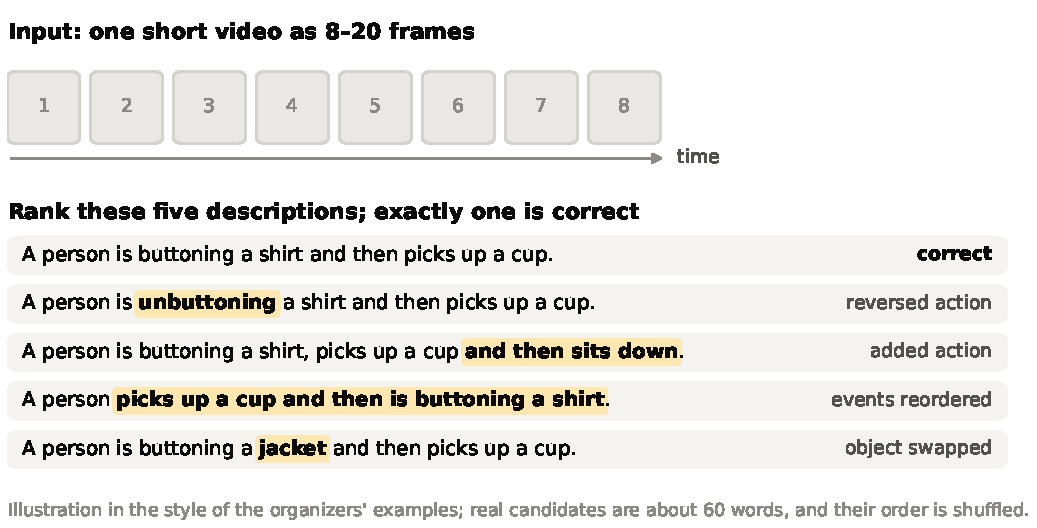
\includegraphics[width=0.82\textwidth]{task}
\caption{One episode. The frames are placeholders and the five sentences are a shortened illustration of the kinds
of differences the organizers showed (a reversed and an added action) and two of our generated kinds; real
candidates are about 60 words and shuffled. Highlighted: the one detail in which each wrong candidate differs.}
\label{fig:task}
\end{figure*}

Four properties of the competition shaped our work:
\begin{itemize}
\item[\cha1] \textbf{No wrong candidates for training.} The 4,170 training episodes have one correct description
  each and no negatives, so wrong candidates must be generated, and local validation measures how well a model
  rejects our generated candidates.
\item[\cha2] \textbf{Near-identical candidates.} A one-word edit of a 60-word description keeps its MPNet sentence
  embedding at cosine similarity 0.983 on average, so a model that compares one text vector with the video can
  barely see the edit; the order of events in the frames often decides.
\item[\cha3] \textbf{Benchmark shift.} The 1,910 test episodes come from a different benchmark, with candidates
  written by a process we could not see.
\item[\cha4] \textbf{Scarce, noisy feedback.} Thirty leaderboard checks on 573 public episodes, each uncertain by
  about $\pm0.016$.
\end{itemize}

We first built video rankers on frozen encoders and generated hard negatives (\cha1, \cha2). They scored about
0.8 locally and near chance publicly. Text-only rules, which ignore the video, then scored far above chance, which
points to annotation artifacts in the test candidates (\cha3). Our final rule fuses two such rankings, using
worst-case bounds computed from per-episode leaderboard results to choose among fusion rules before uploading
(\cha4). This report describes what we tried, what worked, and why the video-based methods did not.

%% ------------------------------------------------------------------------------------------------------------------
\section{Related Work}

Video-language models often fail to distinguish the order of events~\cite{bagad2023testoftime}, and hard negatives
that change the verb of a caption improve verb understanding~\cite{momeni2023verbs}; our generated negatives follow
the same idea. The training videos come from the Perception Test benchmark~\cite{patraucean2023perception}. The
competition permitted four pretrained models: DINOv2~\cite{oquab2023dinov2} for images, an MPNet~\cite{song2020mpnet}
sentence encoder trained as in Sentence-BERT~\cite{reimers2019sbert}, SigLIP~\cite{zhai2023siglip} for image-text
matching, and SmolVLM~\cite{marafioti2025smolvlm} as a vision-language model. In natural language inference,
models that see only the hypothesis beat chance because of annotation artifacts~\cite{gururangan2018artifacts,poliak2018hypothesis};
our text-only rules play the role of such a hypothesis-only baseline. Selecting the candidate most similar to the
others is the minimum Bayes risk decision rule with a similarity utility~\cite{kumar2004mbr}.

%% ------------------------------------------------------------------------------------------------------------------
\section{Data and Evaluation Protocol}

The organizers' training descriptions are 42--75 words long (median 60) and were written from the frames by a
language model, according to their documentation. We split the training episodes 80:20 by episode with a fixed
seed, which leaves 834 validation episodes, and never train on them.

\paragraph{Generated negatives (\cha1).} Each validation episode gets its correct description and four negatives
of one kind, in random order, so that tied scores never favour a position. We generate seven kinds from the
organizers' descriptions with code and a fixed seed, and none from hand-written text
(Table~\ref{tab:negatives}). Because we choose the negatives, a model can learn how a negative was made instead of
what the video shows. To detect this, we train a text-only classifier on each kind, a hypothesis-only baseline:
above about 0.42 it finds the correct description without the video, so the kind gives the answer away
(Table~\ref{tab:negatives}, last column). Added actions are always longer, and the shortest candidate is correct
every time.

\begin{table}[t]
\caption{Kinds of generated negatives and the score of a text-only classifier on each (validation, chance
0.375). A score well above chance means the kind can be told apart without the video.}
\label{tab:negatives}
\footnotesize
\setlength{\tabcolsep}{3pt}
\begin{tabularx}{\columnwidth}{>{\raggedright\arraybackslash}p{1.75cm}>{\raggedright\arraybackslash}Xr}
\toprule
Kind & How it is made & Text only \\
\midrule
Random & another episode's description & 0.370 \\
Lexical & a nearest description by word overlap, with hubness reduction (CSLS~\cite{conneau2018csls}) & 0.397 \\
Similar episode & a description of an episode with overlapping action labels & 0.398 \\
Reorder & the sentences after the opening in another order & 0.451 \\
Swapped action & one sentence replaced by a sentence from another description & 0.544 \\
Added action & a sentence from another description inserted & 0.995 \\
Word swap & one word replaced by a word found in the same contexts & -- \\
\bottomrule
\end{tabularx}
\end{table}

\paragraph{The leaderboard (\cha4).} The public leaderboard scores 573 episodes, so one score is uncertain by about
$\pm0.016$; comparisons of two submissions on the same episodes are tighter (paired noise 0.005--0.013). The site
returned the rank of the correct description in each episode. We used these per-episode results only in aggregate,
to compare and simulate rules, never to tune to single episodes. Even so, the final rule was chosen with public
results, so its public score is optimistic; the private leaderboard, 1,337 episodes we never saw, is the unbiased
measure.

\paragraph{Rules followed.} Only the four permitted models were used, with no distillation from any other model.
Generative augmentation used a local Qwen3-4B-Instruct model that runs on one T4, as the rules require; no external
AI service generated data. Inference for all 1,910 test episodes had to finish within 15 minutes on one T4.

%% ------------------------------------------------------------------------------------------------------------------
\section{Video-Based Ranking}

\paragraph{Trained rankers (\cha1, \cha2).} The organizers' baseline encodes each frame with DINOv2 and the
description with MPNet, mean-pools the frames, and trains an MLP on the concatenation, with both encoders frozen.
We replaced its binary loss with a listwise ranking loss over one correct and several generated negatives, added
temporal layers over the frames and cross-attention from text to frames, and trained on reversed frames paired with
the reversed description (flipping) so that the model must use frame order (Table~\ref{tab:rankers}). The
validation score rose from 0.690 to 0.791 on the two kinds of negatives without a text cue, and the share of
reversed-frame pairs where the model changes its choice rose from chance to 0.728. Publicly, these models scored
0.35--0.40.

\begin{table}[t]
\caption{Trained video rankers, each row adding one change. Clean: mean validation score on the two negative kinds
without a text cue (similar episode, lexical). Order: share of pairs where reversing the frames flips the model's
choice between a description and its reversed version (chance 0.5). Public: leaderboard, where uploaded.}
\label{tab:rankers}
\footnotesize
\setlength{\tabcolsep}{3pt}
\begin{tabularx}{\columnwidth}{>{\raggedright\arraybackslash}Xccc}
\toprule
Model & Clean & Order & Public \\
\midrule
Organizers' baseline & 0.690 & $\approx$0.5 & 0.3469 \\
Listwise ranking loss$^{a}$ & 0.761 & 0.500 & -- \\
+ hard negatives & 0.730 & 0.500 & -- \\
+ temporal layers & 0.766 & 0.569 & -- \\
+ cross-attention, reverse loss, flipping & 0.781 & 0.668 & -- \\
+ lexical negatives & 0.791 & 0.728 & 0.3586 \\
+ word-swap negatives & -- & -- & 0.3968 \\
\bottomrule
\end{tabularx}
\par\smallskip\footnotesize $^{a}$Also changes the learning rate, batch size and number of negatives.
\end{table}

\paragraph{Zero-shot SigLIP (\cha2).} SigLIP reads at most 64 tokens, so we score each sentence against its best
frame and average over sentences. It separates candidates from different scenes well (0.978 against random
negatives) but falls below chance on word swaps and reorderings (0.423 and 0.324), because whole-sentence matching
cannot see a one-word edit or the order of events. Added to the medoid ranking of Section~\ref{sec:text} with equal
weight, it lowered the public score to 0.4682 (Table~\ref{tab:public}).

\paragraph{SmolVLM on the differing tokens (\cha2).} To make the vision-language model look at the edit, we score
only the tokens where candidates differ, as the log-probability of each token given the frames minus that without
them. With the right video it prefers the correct candidate in 62.5\% of word-swap pairs, and with another
episode's video in 46.3\%, so it reads the video, weakly. Added to the medoid ranking with equal weight, it scored
0.5044 publicly. A SmolVLM fine-tuned to separate one-word edits, allowed to overrule the medoid ranking only when
confident, changed 49 public episodes: 16 for the better and 33 for the worse.

\paragraph{Monotonic event-to-frame alignment (\cha2).} Order differences need order evidence, so we split each
candidate into events, score every event against every frame with SigLIP, and compare the best total when events
take frames in their stated order (dynamic programming, as in dynamic time warping) with the total when they need
not. Without training, it ranks reorderings at 0.495 with the right video against 0.367 with a wrong one. Alone it
scored 0.4295 publicly, above chance, but part of that comes from a preference for candidates with fewer events; as
the ranking for places three to five after the text rules, it changed the score by $-0.0044$, within the noise.

%% ------------------------------------------------------------------------------------------------------------------
\section{Text-Only Ranking}\label{sec:text}

\begin{figure*}[t]
\centering
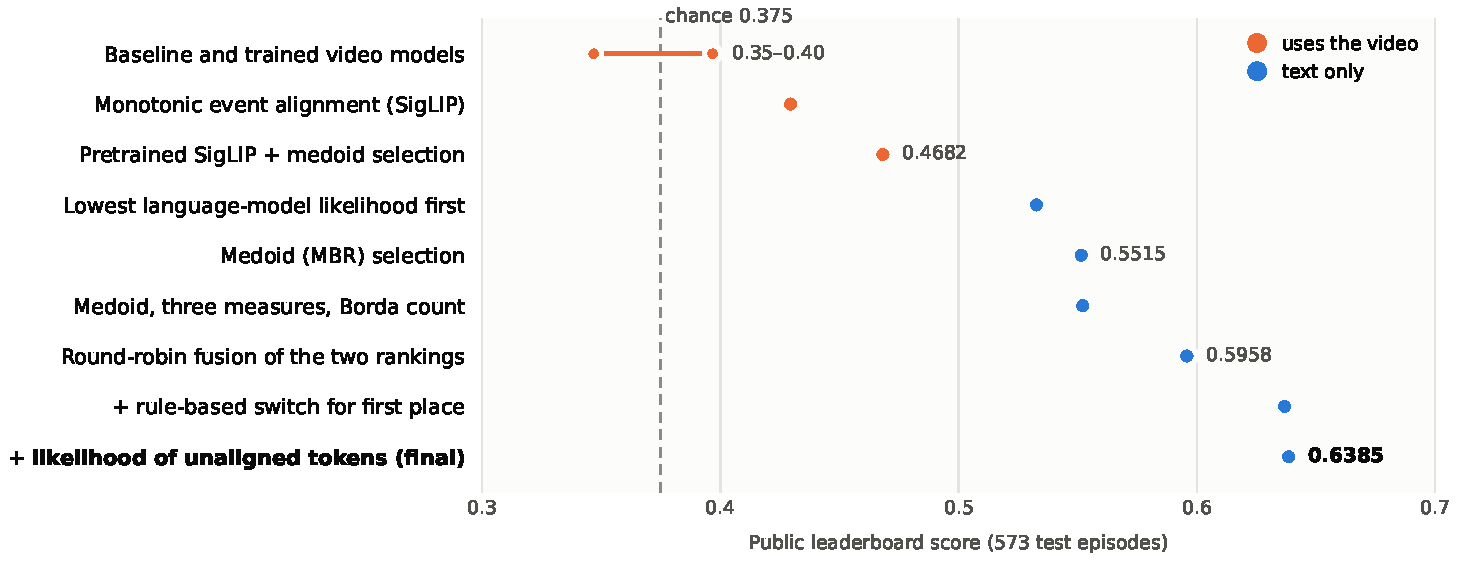
\includegraphics[width=0.8\textwidth]{scores}
\caption{Public leaderboard score at each step. Every method that uses the video (orange) stays below the
text-only rules (blue); the final rule scores 0.6385, and 0.6417 on the private leaderboard.}
\label{fig:scores}
\end{figure*}

\paragraph{Medoid selection (\cha3).} If the four wrong candidates are edits of the correct one, the correct
description is the one most similar to all the others: the medoid of the five, or the minimum Bayes risk choice
with a similarity utility~\cite{kumar2004mbr}. We rank candidates by their mean word-sequence similarity to the
other four, which needs no training and no video. It scored 0.5515 publicly, ranking the correct description first
in 40.8\% of episodes. Fusing three similarities (token overlap, MPNet cosine, word-sequence similarity) by the sum
of their ranks, a Borda count, scored 0.5521, the same within the noise (paired difference $+0.0007$, 95\%
interval $[-0.019, +0.020]$).

\paragraph{Lowest language-model likelihood (\cha3).} We also ranked candidates by the mean log-probability of
their word pairs under an interpolated bigram model fitted on the training descriptions. Most likely first scored
0.2411, far below chance (Table~\ref{tab:public}), so on the test the correct description reads \emph{less} like
the training text than the wrong ones do. Our generated negatives behave the opposite way: there, edits make the
wording less likely. Ranking least likely first gives 0.5327, and its per-episode scores are uncorrelated with the
medoid ranking's ($r=-0.008$). We do not know why the direction is reversed.

\paragraph{Fusing the two rankings (\cha4).} Summing the two rankings scored 0.5443, below the medoid ranking alone.
The per-episode results give the correct description's rank under each rule, but not the wrong candidates' places,
so we computed each fusion rule's score over all placements of the wrong candidates consistent with those ranks
(Table~\ref{tab:fusion}). Round-robin fusion, which takes the next unused candidate from each ranking in turn, scored
highest in the simulation, and its worst case, 0.5639, was already above both rankings alone. It scored 0.5958
publicly.

\begin{table}[t]
\caption{Fusing the Borda-count medoid ranking with lowest likelihood, simulated from public per-episode ranks
before uploading. Simulated: wrong candidates placed with the overlap that reproduces the observed rank sum.
Worst case: minimum over every consistent placement.}
\label{tab:fusion}
\footnotesize
\begin{tabularx}{\columnwidth}{>{\raggedright\arraybackslash}Xcc}
\toprule
Fusion rule & Simulated & Worst case \\
\midrule
Round-robin & 0.6016 & 0.5639 \\
Likelihood from public rank shares & 0.5912 & -- \\
Reciprocal-rank points & 0.5696 & -- \\
Rank sum & 0.5394 & -- \\
\midrule
Round-robin, uploaded & \multicolumn{2}{c}{0.5958 (public)} \\
\bottomrule
\end{tabularx}
\end{table}

\paragraph{A rule-based switch for first place (\cha3).} Round-robin fusion still lets the medoid ranking pick
first. The medoid is right when the correct description is the source of the edits, but not when the wrong
candidates are edits of a text that is not among the five. We therefore let the likelihood ranking pick first
when no candidate has all its words in the others, that is, when no candidate looks like the source. On synthetic
candidate sets, the switch leaves the medoid choice alone in every set where the correct description is the source,
and fires in 99\% of sets built from one-word edits of a hidden text. It raised the public score by $+0.041$, to
0.6368, beyond the paired noise. Firing it more often, also when edit distances do not add up, lowered the score
to 0.6206.

\paragraph{Final rule.} When the switch fires, every candidate has words that match nothing in the others. Scoring
only the word pairs that touch these unaligned tokens, the candidate's edit span, gave 0.6385, a change of
$+0.0017$ that is within its paired noise of about 0.007. It became the final because it had the highest public
score. The rule runs in about 0.02\,s per episode.

%% ------------------------------------------------------------------------------------------------------------------
\section{Results}

\begin{table}[t]
\caption{Public leaderboard (573 episodes, chance 0.375, about $\pm0.016$ per score). Video: whether the method
uses the frames. Rank 1 / 5: share of episodes with the correct description first / last, where the per-episode
results were available.}
\label{tab:public}
\footnotesize
\setlength{\tabcolsep}{2.5pt}
\begin{tabularx}{\columnwidth}{>{\raggedright\arraybackslash}Xccc}
\toprule
Method & Video & Public & Rank 1 / 5 (\%) \\
\midrule
Most likely first & no & 0.2411 & 10.5 / 35.3 \\
Trained video rankers (Table~\ref{tab:rankers}) & yes & 0.35--0.40 & -- \\
Event alignment alone & yes & 0.4295 & -- \\
SigLIP + medoid, equal weight & yes & 0.4682 & -- \\
SmolVLM differing tokens + medoid & yes & 0.5044 & -- \\
Least likely first & no & 0.5327 & 35.3 / 10.5 \\
SmolVLM overruling the medoid & yes & 0.5382 & 38.7 / 11.0 \\
Rank sum: medoid + least likely & no & 0.5443 & 35.3 / 7.3 \\
Medoid selection & no & 0.5515 & 40.8 / 11.3 \\
Medoid, Borda count of three & no & 0.5521 & 41.7 / 13.8 \\
Round-robin fusion & no & 0.5958 & -- \\
+ rule-based switch & no & 0.6368 & -- \\
+ unaligned tokens (final) & no & \textbf{0.6385} & -- \\
\bottomrule
\end{tabularx}
\end{table}

Table~\ref{tab:public} and Figure~\ref{fig:scores} give the public scores. No method that uses the video beat the
best text-only rule, and every combination in which the video could move the text ranking scored lower than the
text ranking alone. Among the text-only rules, the steps that changed which candidate is ranked first gained most:
round-robin fusion added $+0.044$ over the Borda-count medoid ranking, and the rule-based switch another $+0.041$.

On the private leaderboard, 1,337 episodes never used for any decision, the final rule scored 0.6417, and 0.6408
on all 1,910 test episodes.\footnote{The organizers reported the combined score; the private score follows from it
and the public score.} The private score is slightly above the public one, so choosing rules with public results
did not overfit the public episodes.

%% ------------------------------------------------------------------------------------------------------------------
\section{Discussion and Limitations}

\paragraph{Why validation misled us (\cha1, \cha3).} Our generated negatives mostly differ from the correct
description in content, and a model passes them by matching the objects in the scene. On the test, all five
candidates describe the same scene, so that skill does not help. The language-model likelihood makes the mismatch
concrete: on our negatives the correct description is the more likely one, on the test it is the less likely one.
Generated validation sets can rank models against each other, but they did not predict the leaderboard.

\paragraph{Annotation artifacts (\cha3).} Two text-only rules beat chance by 0.18 and 0.16, and the final rule
by 0.26. As in natural language inference~\cite{gururangan2018artifacts,poliak2018hypothesis}, this shows that how the
candidates were written gives the answer away in part. We attribute the medoid's success to wrong candidates that
are edits of a common text, and we do not know what makes the correct description less likely under the training
text's language model.

\paragraph{Limitations.} The final rule does not use the video, so it does not solve the task as intended, and it
depends on how this test set's candidates were written; a test built differently would likely defeat it. Our
analysis of the test candidates is indirect, because we never saw their text. Each video method was trained or
tuned once, with one seed for most runs, under the competition's time limit. The one video signal with real order
information, the monotonic alignment, was weak alone; whether a stronger version would complement the text rules
is untested.

%% ------------------------------------------------------------------------------------------------------------------
\section{Conclusion}

On a video ranking task with near-identical candidates and a benchmark shift, every video-based method we built
stayed near chance, while two text-only rules, medoid selection and lowest language-model likelihood, were
uncorrelated and far above it. Round-robin fusion of the two, a rule-based switch for first place, and worst-case
bounds to choose among fusions before uploading gave 0.6385 public and 0.6417 private. Two lessons carry over:
validate on candidates made the way the test candidates are made, and measure a hypothesis-only baseline before
crediting a model with reading the video.

\bibliographystyle{plainnat}
\bibliography{references}

\appendix
\section{Reproduction}
The code, the experiment log and the Colab notebook that built the final submission are at
\url{https://github.com/naufalkmd/fine-grained-multimodal-video-ranking}. The final submission is rebuilt with
\texttt{notebooks/final\_text\_colab.ipynb} on a T4 in about 20 minutes from the organizers' training data, which
we cannot redistribute.

\end{document}
